\chapter{Interfaz gráfica (GUI)}

Se implementó una interfaz gráfica de forma tal de ejecutar el sistema implementado de forma más práctica. Tanto para el proceso de principio a fin, como para cada bloque por separado.

Esto último permite obtener los datos de salida de cada bloque sin necesidad de ejecutar el proceso entero ahorrando tiempo de procesamiento.

Como era de esperarse, la interfaz gráfica tiene, entre otras cosas, todos los parámetros que se le ingresan al proceso en cada módulo por ejemplo: umbral fijo y filtro de área en el bloque de detección, marcadores totales, cámaras a utilizar en la reconstrucción, o el rango de frames donde se procesarán los marcadores.

En la Figura \ref{guiVent} se observa una captura de pantalla de la interfaz implementada.

\begin{figure}[H]
\hspace{-1cm}
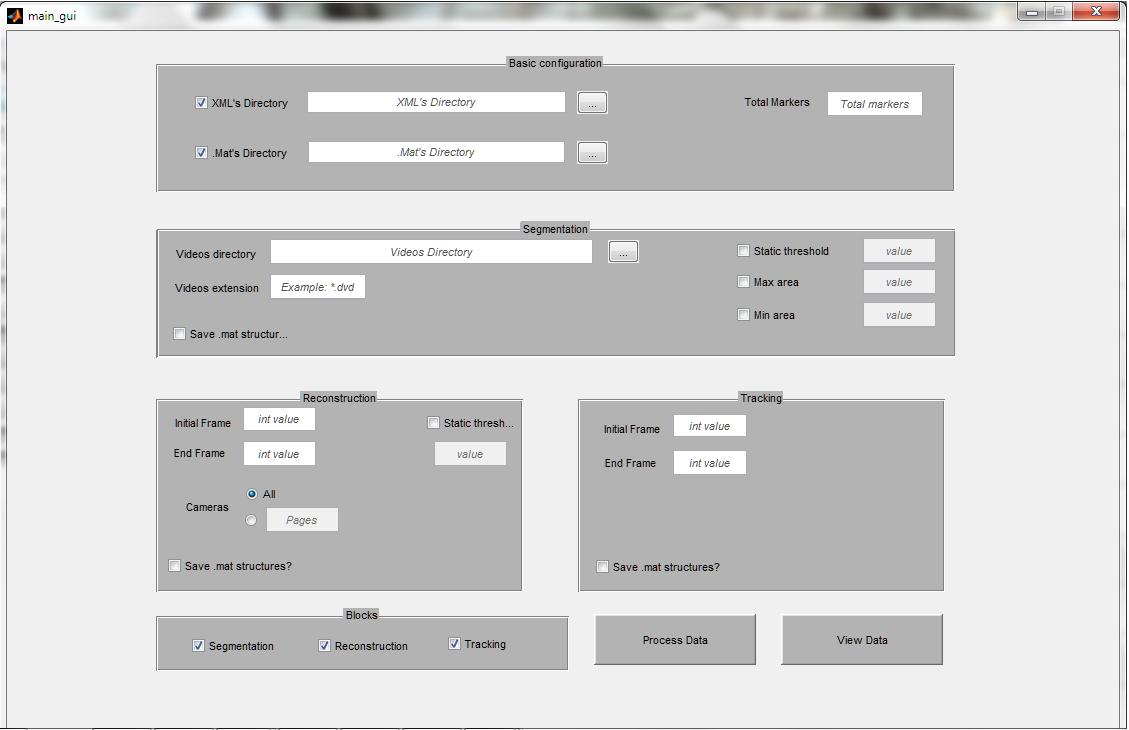
\includegraphics[scale=0.54]{img/gui.png}
\caption{Vista de la interfaz gráfica implementada.}
\label{guiVent}
\end{figure}

Cabe destacar que esta interfaz no pretende ser la interfaz final de la aplicación, sino un bosquejo, ya que el estado actual del sistema no permite que sea definido como ``aplicación de usuario'' sino como el estudio e implementación de un sistema de captura de movimiento diseñado previamente.

Queda como pendiente, preferiblemente para un proyecto de ingeniería de sistemas, diseñar una interfaz de usuario completa, amigable y con mejor usabilidad para los especialistas que utilizarán el sistema.